\chapter{Caches and Cache Coherence}
\label{ch:coherence}

\newcommand{\Cread}{\textit{C\_read}}
\newcommand{\Cwrite}{\textit{C\_write}}

Shared memory is attractive because processors communicate through ordinary reads and writes. But
every modern processor has caches, and caches break the simple picture of ``one memory that everybody sees''.
This chapter explains how, and how hardware repairs it.

\section{Caches in a multiprocessor}
\slides{8--9}

Recall from your Chapter~1 that a cache holds \emph{copies} of small blocks of main memory, called
\term{cache lines} (or blocks), which are the unit of transfer between memory and cache. On current
processors a line is $64$~bytes. A read that finds its line in the cache is a \emph{hit} and takes a few cycles; one that does not is a
\emph{miss}, and the whole line is fetched from the next level.

In a multicore chip each core has its \emph{own private} cache (typically at least the first level, often also the second), and there may be a shared last-level cache. The private caches are where the trouble comes from.

\begin{center}
\begin{tikzpicture}
  \foreach \i in {1,2,3} {
     \node[pe] (p\i) at (\i*2.3,2.4) {$P_\i$};
     \node[ca] (c\i) at (\i*2.3,1.6) {cache $C_\i$};
     \draw[lnk] (p\i) -- (c\i);
  }
  \node[busbar,minimum width=7.4cm] (bus) at (4.6,0.8) {shared bus / interconnect};
  \node[mm,minimum width=7.4cm] (mem) at (4.6,0) {main memory};
  \foreach \i in {1,2,3} \draw[lnk] (c\i) -- (c\i |- bus.north);
  \draw[lnk] (bus) -- (mem);
\end{tikzpicture}
\end{center}

\subsection{Write policies: what happens on a write?}
\label{sec:writepolicy}

Reads are simple: if the line is in the cache, use it. Writes raise a question: the cache now holds a
\emph{newer} value than main memory. What should happen to memory? There are two classical answers.

\begin{definition}{write-through and write-back}
\textbf{Write-through}: every write updates the cache \emph{and} main memory immediately. Memory is never out of
date, but every write generates memory traffic.\\
\textbf{Write-back}: a write updates only the cache and sets a \term{dirty bit} on that line to record that it
differs from memory. The line is written back to memory only later, when it is \emph{evicted} (thrown out to make room for another
line). Repeated writes to the same line then cost nothing extra.
\end{definition}

Most caches are write-back, because it saves a great deal of memory bandwidth. A related detail: on a
\emph{write miss}, a write-back cache usually first fetches the whole line (\emph{write-allocate}) and then modifies it,
since the rest of the line must be valid in the cache. We will see that the ``Dirty'' state in the coherence protocol
below is the multiprocessor version of this dirty bit.

\begin{intuition}
Imagine a shared recipe book in the library (main memory) and a photocopy of one page on your desk (your cache). If you
scribble a correction on your copy, the library's page does not change until you walk back and
update it (write-back). Meanwhile a friend with their own photocopy of the same page has no idea about your correction. This is the problem
of the next section.
\end{intuition}

\section{The cache coherence problem}
\slides{9--10}

\begin{workedex}{stale data}
A variable $X$ is in main memory with the value $0$.
\begin{center}
\small
\begin{tabular}{@{}clccc@{}}
\toprule
Step & Event & $P_1$'s cache & $P_2$'s cache & Memory\\
\midrule
0 & initially & --- & --- & $X=0$\\
1 & $P_1$ reads $X$ (miss, line fetched) & $X=0$ & --- & $X=0$\\
2 & $P_2$ reads $X$ (miss, line fetched) & $X=0$ & $X=0$ & $X=0$\\
3 & $P_1$ writes $X=1$ (hit, only cache updated) & $X=1$ & $X=0$ & $X=0$\\
4 & $P_2$ reads $X$ (\textbf{hit}) returns \textbf{0} & $X=1$ & $X=0$ & $X=0$\\
\bottomrule
\end{tabular}
\end{center}
In step~4, $P_2$ hits in its own cache and gets $0$, although the latest value written is $1$. The slide marks
exactly this: ``Cache hit: wrong data!!''. The value $0$ in $P_2$'s cache is called \term{stale}.
\end{workedex}

\begin{pitfall}
Write-through does not solve this. With write-through, memory would hold $1$ after step~3, but $P_2$'s \emph{copy} would still say $0$ and
$P_2$ would still hit on it. The problem is not main memory but the existence of \emph{several copies}.
\end{pitfall}

\begin{definition}{cache coherence}
A memory system is \emph{coherent} if, for every individual memory location, the following hold:
\begin{enumerate}
  \item \textbf{Program order.} A read by a processor that follows its own write to the location returns that
        write's value (unless another processor wrote in between).
  \item \textbf{Coherent view.} A read returns a value written by another processor if the write happened
        ``long enough ago'': writes do not stay invisible forever.
  \item \textbf{Write serialisation.} Writes to the same location are seen in the \emph{same order} by all
        processors. If $P_1$ writes $1$ and $P_2$ writes $2$, it cannot happen that one processor sees $1$ then $2$
        while another sees $2$ then $1$.
\end{enumerate}
The slide's one-line version: processes shouldn't read ``stale'' data.
\end{definition}

\begin{keyidea}
A coherent system behaves, \emph{per location}, as if there were just one copy of that location.
\end{keyidea}

\begin{pitfall}
\textbf{Coherence is not consistency.} Coherence is about the order of operations on \emph{one} location.
\emph{Memory consistency} is about the order in which operations on \emph{different} locations become visible, and it
is what programs depend on in code like this (initially \cl{data = flag = 0}):
\begin{center}
\begin{tabular}{@{}l|l@{}}
$P_1$ & $P_2$\\ \hline
\cl{data = 42;} & \cl{while (flag == 0) ;}\\
\cl{flag = 1;} & \cl{print(data);}\\
\end{tabular}
\end{center}
You would expect $42$ to be printed; whether this is guaranteed depends on the machine's \emph{consistency model}.
Consistency models are a separate topic that this course does not examine in depth. Everything below concerns coherence only.
\end{pitfall}

\textbf{Who fixes it?} In principle software could do it: the compiler or operating system could mark shared data as uncacheable or
flush caches at the right times. This would be slow and a nightmare to program. The
slides give the standard answer: \emph{hardware} coherence mechanisms, invisible to the program.

\section{Update versus invalidate}
\slides{11--12}

When a processor writes a line that other caches also hold, those other copies must be dealt with. There are two policies:

\begin{definition}{write-update and write-invalidate}
\textbf{Write-update}: on every write, the new value is broadcast to all caches holding the line, and they
overwrite their copies. \\
\textbf{Write-invalidate}: on a write, the writer sends a short message that makes the other caches mark their copies
\emph{invalid}. A processor that later needs the line takes a miss and fetches the fresh value.
\end{definition}

The slide asks: which is better? Compare them on two access patterns.

\begin{workedex}{one writer, no readers}
$P_1$ writes the same variable $100$ times in a row; $P_2$ holds a copy but never looks at it again.
\begin{itemize}
  \item \textbf{Update:} $100$ broadcasts, each carrying data, although nobody needs them.
  \item \textbf{Invalidate:} the first write invalidates $P_2$'s copy ($1$ message). $P_1$ now holds the only valid copy,
        and the other $99$ writes hit locally with no bus traffic at all.
\end{itemize}
\end{workedex}

\begin{workedex}{tight producer--consumer}
$P_1$ writes a value, $P_2$ reads it, $P_1$ writes the next value, $P_2$ reads it, and so on.
\begin{itemize}
  \item \textbf{Update:} each write is broadcast and $P_2$'s read hits. One transaction per round, with a fast read.
  \item \textbf{Invalidate:} each write invalidates $P_2$'s copy, and $P_2$'s read then misses and must fetch the line.
        Two transactions per round and a slow read.
\end{itemize}
\end{workedex}

\begin{center}
\small
\begin{tabularx}{\linewidth}{@{}l X X@{}}
\toprule
 & \textbf{Write-update} & \textbf{Write-invalidate}\\
\midrule
Write cost & high: data broadcast on every write & low: a short invalidation, and only for the first write\\
Read after a remote write & fast: copy already updated & slow: miss, fetch the line\\
Wasted traffic & updates to caches that never read again & none for data that is not re-read\\
Multi-word lines & each word written is a separate update & one invalidation covers the whole line\\
Best for & one-to-one producer--consumer on a single word & most real programs\\
\bottomrule
\end{tabularx}
\end{center}

Most programs write a variable many times before anyone else reads it, and data is usually written in
runs to neighbouring words of the same line, so \textbf{write-invalidate dominates in practice} and is what the
rest of the course (and almost all hardware) assumes.

\section{The three-state invalidate protocol}
\slides{12--14}

A coherence \term{protocol} is a set of rules that every cache controller follows so that the whole system stays coherent. It works
line by line: \emph{each line in each cache} has a \emph{state}, and the state changes in response to events.
Note: the state belongs to the pair (cache, line), not to a variable or to a processor in general.

\subsection{The states}

The slides use three states (the textbook name for this protocol is \textbf{MSI}, with Modified
for the slide's Dirty):

\begin{definition}{the three states}
\textbf{I -- Invalid}: this cache has no valid copy of the line (it was never loaded or another processor has updated the data).\\
\textbf{S -- Shared}: this cache has a valid copy, \emph{read-only}, and other caches may also have copies. Memory is up to date.\\
\textbf{D -- Dirty} (Modified in textbooks): this cache has the \emph{only} valid copy and it has been modified. Memory is
\emph{stale}.
\end{definition}

\begin{keyidea}
The protocol maintains the \emph{single-writer, multiple-reader} rule. For any line, at any moment either
(a) any number of caches hold it in S (and none in D), or (b) exactly one cache holds it in D and all others have it invalid.
\end{keyidea}

\subsection{The events}

Two kinds of events change a line's state:
\begin{itemize}
  \item \textbf{Events from this cache's own processor}: \emph{read} and \emph{write}.
  \item \textbf{Events observed from other processors} (the dashed arrows in the slide's diagram):
        \Cread{} means ``another processor is reading this line'', and \Cwrite{} means ``another processor is writing
        this line'' (it wants exclusive ownership).
\end{itemize}

\subsection{The state diagram}

\begin{center}
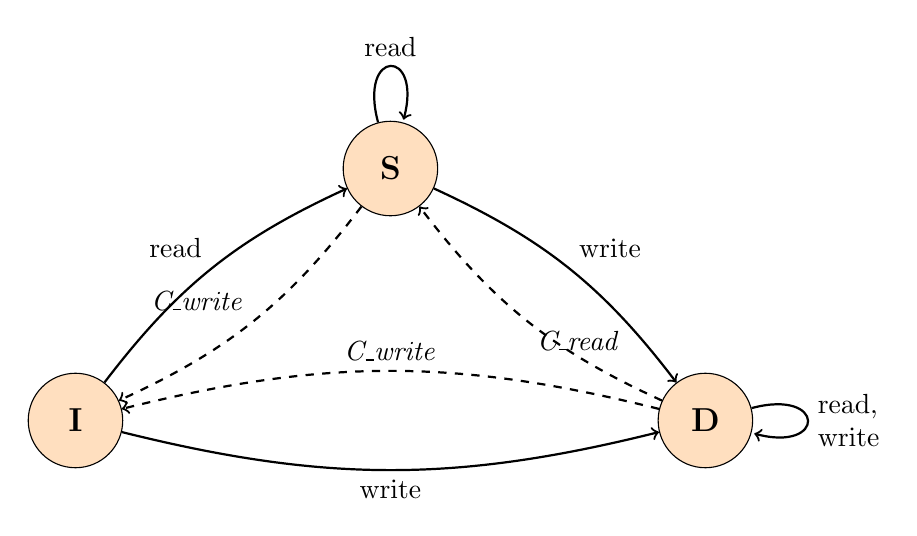
\begin{tikzpicture}[st/.style={circle,draw,fill=orange!25,minimum size=12mm,font=\bfseries\large},scale=1.0]
  \node[st] (S) at (0,3.2) {S};
  \node[st] (I) at (-4,0) {I};
  \node[st] (D) at (4,0) {D};
  \path[->,thick]
    (S) edge[loop above] node[above]{read} (S)
    (D) edge[loop right] node[right,align=left]{read,\\write} (D)
    (I) edge[bend left=14] node[above left]{read} (S)
    (S) edge[bend left=14] node[above right]{write} (D)
    (I) edge[bend right=14] node[below]{write} (D);
  \path[->,thick,dashed]
    (S) edge[bend left=14] node[above left]{\Cwrite} (I)
    (D) edge[bend left=14] node[below right]{\Cread} (S)
    (D) edge[bend right=14] node[above]{\Cwrite} (I);
\end{tikzpicture}
\end{center}

Solid arrows are caused by this cache's own processor; dashed arrows are caused by what \emph{other} processors do.
(Events not drawn leave the state unchanged: for example, \Cread{} on a line in S keeps it in S, and \Cread{} or
\Cwrite{} on a line in I does nothing.)

\subsection{Reading the diagram, one arrow at a time}

\begin{center}
\small
\begin{tabularx}{\linewidth}{@{}c l c X@{}}
\toprule
\textbf{From} & \textbf{Event} & \textbf{To} & \textbf{What the hardware does}\\
\midrule
S & read & S & Hit. Nothing leaves the cache.\\
S & write & D & The cache must become the sole owner. It broadcasts an \emph{invalidate}; every other copy goes S$\to$I (their \Cwrite{}). No data transfer is needed, since this cache already holds the line.\\
S & \Cwrite & I & Another processor is writing: drop this copy.\\
I & read & S & Read miss. The line is fetched from memory, or from the cache that holds it in D (see below). Cache ends in S.\\
I & write & D & Write miss. The line is fetched \emph{with intent to modify}, all other copies are invalidated, and the cache ends in D.\\
D & read, write & D & Hits. This cache is the sole owner, so no bus traffic at all.\\
D & \Cread & S & Another processor wants to read. This cache holds the only up-to-date data, so it \emph{supplies} the line (and memory is updated); both caches then hold the line in S.\\
D & \Cwrite & I & Another processor wants to write. This cache supplies the data and invalidates its own copy: the other cache becomes the single owner (D).\\
\bottomrule
\end{tabularx}
\end{center}

\begin{pitfall}
When a line is Dirty somewhere, \emph{memory is stale}. A processor that misses on such a line must \textbf{not} read it from memory; it must get it from the owning
cache. This is why the transitions D$\to$S and D$\to$I involve the owner supplying data.
\end{pitfall}

\subsection{A complete trace}

\begin{workedex}{two processors, one variable}
Line containing $X$ is in memory with $X=0$; both caches start in I. Write-back, as above.
\begin{center}
\small
\begin{tabular}{@{}cllllll@{}}
\toprule
 & Event & $P_1$ & $P_2$ & Memory & Bus activity\\
\midrule
0 & start & I & I & $0$ & ---\\
1 & $P_1$ reads $X$ & S ($0$) & I & $0$ & read miss, line from memory\\
2 & $P_2$ reads $X$ & S ($0$) & S ($0$) & $0$ & read miss, line from memory\\
3 & $P_1$ writes $X{=}5$ & D ($5$) & I & $0$ (stale) & invalidate sent; $P_2$: S$\to$I\\
4 & $P_2$ reads $X$ & S ($5$) & S ($5$) & $5$ & read miss; $P_1$ (D) supplies line, D$\to$S\\
5 & $P_2$ writes $X{=}7$ & I & D ($7$) & $5$ (stale) & invalidate sent; $P_1$: S$\to$I\\
6 & $P_1$ reads $X$ & S ($7$) & S ($7$) & $7$ & read miss; $P_2$ (D) supplies line, D$\to$S\\
\bottomrule
\end{tabular}
\end{center}
Notice that step~4 returns $5$, not the stale $0$, and step~6 returns $7$: coherence is restored. The invariant (single writer or many
readers) holds after every step. Steps~3 and 5 have the memory stale; no processor can read it by mistake,
because a processor that misses is served by the owner.
\end{workedex}

\subsection{Beyond three states (not on the slides, but you will meet the names)}

\begin{itemize}
  \item \textbf{MESI} adds \textbf{E (Exclusive)}: a clean line that this cache holds and no other cache does. It matters
        because most data is private. In MSI, reading a private line then writing it needs two steps: I$\to$S on the read, then an
        invalidation broadcast on the write. In MESI the read brings the line in as E, and the first write moves E$\to$D \emph{silently},
        with no bus transaction.
  \item \textbf{MOESI} adds \textbf{O (Owned)}: a dirty line that is shared. The owner supplies data to readers and
        memory need not be updated at every read, saving memory traffic.
\end{itemize}

\textbf{A caution about the diagram.} It shows transitions as if they were instantaneous. In real hardware two processors may try to write
the same line at the same time, and the controllers must order these events consistently. This is exactly what the bus provides in a snooping system (next
section) and what the directory does in a directory system.

\section{Implementing coherence: snooping and directories}
\slides{15--17}

The protocol is the \emph{rules}; the \emph{implementation} decides how cache controllers learn about each other's actions.
There are two main designs.

\subsection{Snooping (bus-based)}

\begin{definition}{snooping protocol}
All caches are attached to a \emph{shared bus}. Every memory operation that matters for coherence
(a miss, an invalidation) is \emph{broadcast on the bus}. Each cache controller continuously watches (``snoops on'') the bus, compares each address against the lines in its own cache, and takes action when it
holds a copy.
\end{definition}

Why this works: the slide says ``there is only one operation through the bus at a time''. The bus is a single shared wire set, so it
automatically puts all transactions in a single order that everyone sees, which gives write serialisation for free. When $P_1$ puts an
invalidation for line $L$ on the bus, every other controller hears it in the same order, invalidates its copy of $L$ if it has one, and
the protocol of the previous section proceeds.

\textbf{Limitations.}
\begin{itemize}
  \item The bus carries one transaction at a time, so it becomes a \emph{bottleneck} as processors are added: every miss and
        invalidation from every processor competes for it.
  \item Every cache must check every bus transaction, which costs energy and cache bandwidth even for lines it does not have.
  \item Electrically, a bus with many attached devices cannot be clocked fast.
\end{itemize}
Snooping is therefore used for small machines (roughly up to a few tens of processors) or within a small group of cores.

\subsection{Directory-based}

\begin{definition}{directory protocol}
A \emph{directory} records, for each memory line, \emph{which caches currently hold a copy} (and whether it is
dirty). On a miss or a write, coherence messages are sent \emph{only to the caches the directory lists}, instead of being
broadcast to everyone.
\end{definition}

The slide says ``a central directory maintains states of cache blocks, associated processors''. Logically there is one directory; in a
large machine it is \emph{physically distributed}, each node keeping the directory entries for the lines in \emph{its own} memory
(the line's \term{home node}). A single physical directory would itself be a bottleneck.

\textbf{Directory entry.} For each line: a state (uncached, shared, or exclusive/dirty) and the
\term{presence bits}: one bit per processor, $1$ if that processor has a copy.

\textbf{How a write to a shared line works.} Suppose a line is cached by $P_2$ and $P_3$, and $P_1$ wants to write it.

\begin{center}
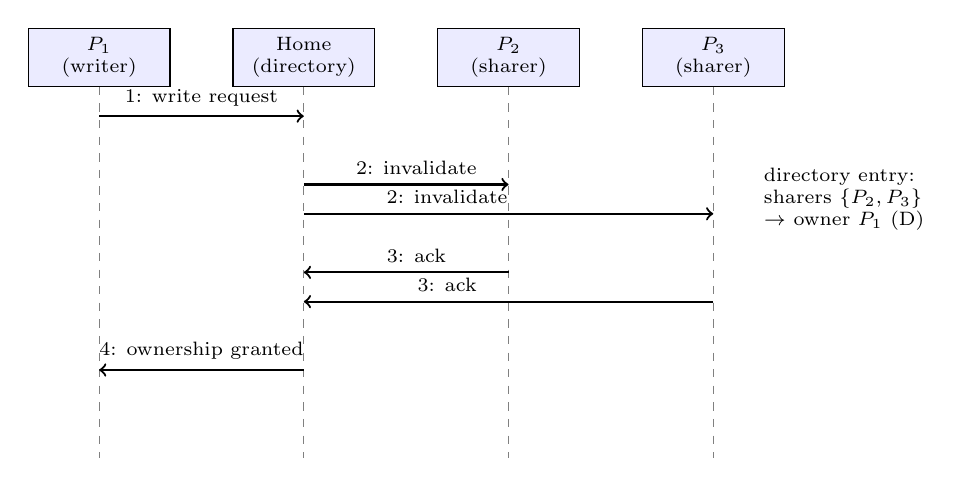
\begin{tikzpicture}[x=2.6cm,y=0.62cm]
  \foreach \x/\n in {0/{$P_1$\\(writer)}, 1/{Home\\(directory)}, 2/{$P_2$\\(sharer)}, 3/{$P_3$\\(sharer)}} {
    \node[draw,fill=blue!8,minimum width=18mm,font=\scriptsize,align=center] (h\x) at (\x,0) {\n};
    \draw[dashed,gray] (\x,-0.6) -- (\x,-8.2);
  }
  \draw[->,thick] (0,-1.2) -- node[above,font=\scriptsize]{1: write request} (1,-1.2);
  \draw[->,thick] (1,-2.6) -- node[above,font=\scriptsize,pos=0.55]{2: invalidate} (2,-2.6);
  \draw[->,thick] (1,-3.2) -- node[above,font=\scriptsize,pos=0.35]{2: invalidate} (3,-3.2);
  \draw[->,thick] (2,-4.4) -- node[above,font=\scriptsize,pos=0.45]{3: ack} (1,-4.4);
  \draw[->,thick] (3,-5.0) -- node[above,font=\scriptsize,pos=0.65]{3: ack} (1,-5.0);
  \draw[->,thick] (1,-6.4) -- node[above,font=\scriptsize]{4: ownership granted} (0,-6.4);
  \node[font=\scriptsize,align=left,anchor=west] at (3.2,-2.9) {directory entry:\\ sharers $\{P_2,P_3\}$\\ $\rightarrow$ owner $P_1$ (D)};
\end{tikzpicture}
\end{center}

Only $P_2$ and $P_3$ are bothered. With $64$ processors a snooping system would have interrupted all $63$ others. In
a \emph{read miss on a line that is dirty in another cache}, the request goes to the home, the home \emph{forwards} it to the
owner, and the owner sends the data to the requester: three steps (hops) instead of the bus's one broadcast. This indirection
is the price paid for scalability.

\subsection{How big is the directory?}

With one presence bit per processor per line (the \term{full bit vector} scheme in the slide), the directory needs
$P$ bits for each of the $M$ memory lines: storage proportional to $M\times P$.

\begin{workedex}{directory overhead}
Memory of $64$~GiB with $64$-byte ($512$-bit) lines has $M = 2^{36}/2^{6} = 2^{30}$ lines.
\begin{itemize}
  \item $P=64$ processors: $2^{30}\times 64$ bits $=8$~GiB, an overhead of $64/512 = 12.5\%$.
  \item $P=1024$ processors: $2^{30}\times 1024$ bits $=128$~GiB, an overhead of $1024/512 = 200\%$: the directory is \emph{larger than the data}.
\end{itemize}
The overhead per line is $P/512$, so it grows linearly with the number of processors. That is the ``but not necessary'' of the slide.
\end{workedex}

\textbf{Why most of that storage is wasted, and the fix.} The total capacity of all caches is tiny compared with memory, so at any moment
\emph{almost every line is in no cache at all} and most of the directory is rows of zeros. And lines that are cached are typically
cached by only a handful of processors. The slide's ``sparse or tagged directory'' and ``limited cache lines and limited presence bits''
exploit this:
\begin{itemize}
  \item \textbf{Sparse (tagged) directory}: keep entries only for lines that are currently cached somewhere, in a small table
        looked up by the line's address (like a cache for directory entries), instead of one entry per memory line.
  \item \textbf{Limited presence information}: instead of $P$ bits, store the identities of at most $k$ sharers (say $k=4$,
        which costs $k\log_2 P$ bits). If a fifth processor wants a copy, the protocol either invalidates one existing sharer, or
        switches to broadcast for that line, or uses a coarse vector (one bit per \emph{group} of processors).
\end{itemize}

\subsection{Snooping versus directory}

\begin{center}
\small
\begin{tabularx}{\linewidth}{@{}l X X@{}}
\toprule
 & \textbf{Snooping} & \textbf{Directory}\\
\midrule
Who learns about a write & everybody (broadcast) & only the listed sharers\\
Interconnect & shared bus (one transaction at a time) & any network, many transactions in parallel\\
Order of writes & provided by the bus & provided by the home node\\
Latency of a miss & short (broadcast) & longer (indirection through the home)\\
Extra storage & none (just the state bits in the caches) & directory ($\propto$ lines $\times$ sharer information)\\
Scalability & tens of processors & hundreds to thousands\\
\bottomrule
\end{tabularx}
\end{center}

Modern multi-socket servers and many-core chips typically use a hybrid: snooping within a small group of cores that
share a cache or a ring, and directory-like structures (or ``snoop filters'') to avoid broadcasting to the rest.

\section{False sharing}
\slides{18--19}

\subsection{The problem}

The protocol operates on whole cache lines. The unit of ownership is a \emph{line} ($64$ bytes), not a variable (typically $4$ or $8$
bytes). The hardware has no idea that a line contains eight different variables.

\begin{definition}{false sharing}
Two processors repeatedly access \emph{different} variables that happen to lie in the \emph{same cache line}, and at least one of them writes.
Logically they share nothing, but the coherence hardware treats the line as shared and moves it back and forth.
\end{definition}

\begin{center}
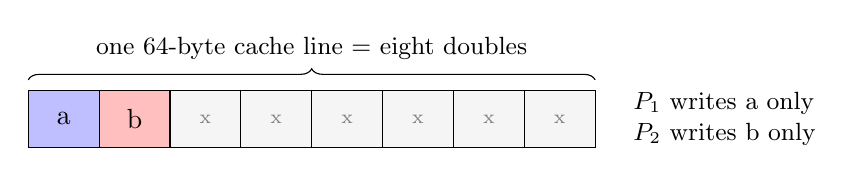
\begin{tikzpicture}[x=0.9cm,y=0.9cm]
  \foreach \i in {0,...,7} { \draw[fill=gray!8] (\i,0) rectangle (\i+1,0.8); }
  \draw[fill=blue!25] (0,0) rectangle (1,0.8); \node at (0.5,0.4) {\cl{a}};
  \draw[fill=red!25]  (1,0) rectangle (2,0.8); \node at (1.5,0.4) {\cl{b}};
  \foreach \i in {2,...,7} \node[font=\scriptsize,gray] at (\i+0.5,0.4) {\cl{x}};
  \draw[decorate,decoration={brace,amplitude=4pt}] (0,0.95) -- (8,0.95) node[midway,above=4pt,font=\small]{one 64-byte cache line = eight doubles};
  \node[font=\small,align=left,anchor=west] at (8.4,0.4) {$P_1$ writes \cl{a} only\\$P_2$ writes \cl{b} only};
\end{tikzpicture}
\end{center}

\begin{workedex}{the line ping-pongs}
$P_1$ repeatedly writes \cl{a} and $P_2$ repeatedly writes \cl{b}, in the same line, with the invalidate protocol:
\begin{enumerate}
  \item $P_1$ writes \cl{a}: line in $P_1$ is D, in $P_2$ is I.
  \item $P_2$ writes \cl{b}: a write miss. The line must be fetched from $P_1$; now $P_2$ is D and $P_1$ is I.
  \item $P_1$ writes \cl{a} again: again a write miss. The line moves back to $P_1$. And so on.
\end{enumerate}
Every write is a miss that needs a transfer across the interconnect (tens to hundreds of cycles) instead of a hit
(a few cycles). The program is correct but can be several times slower than it should be, and it often gets \emph{slower} as threads are added.
\end{workedex}

\textbf{True versus false sharing.} If the two processors accessed the \emph{same} word, the communication would be real
(\emph{true sharing}) and unavoidable. False sharing is an artifact of data layout, and therefore it can be removed.

\subsection{An example in code}

A very common way to get false sharing: each thread keeps its running total in its own element of a shared array.

\begin{lstlisting}
#define NT 8
double partial[NT];                       /* 8 doubles = 64 bytes = ONE cache line */

#pragma omp parallel num_threads(NT)
{
    int t = omp_get_thread_num();
    for (long i = t*(N/NT); i < (t+1)*(N/NT); i++)
        partial[t] += a[i];               /* every iteration writes the shared line */
}
\end{lstlisting}

All eight elements of \cl{partial} sit in one line. Every update by any thread invalidates the line in the other seven caches.
Two fixes:

\begin{lstlisting}
/* Fix 1 (best): accumulate in a private variable, write once at the end */
{   double local = 0.0;
    for (long i = t*(N/NT); i < (t+1)*(N/NT); i++) local += a[i];
    partial[t] = local;                   /* one write per thread */
}

/* Fix 2: padding - make each thread's slot occupy its own cache line */
typedef struct { double v; char pad[56]; } padded_t;      /* sizeof = 64 bytes */
_Alignas(64) padded_t partial2[NT];
/* ... partial2[t].v += a[i]; ... */
\end{lstlisting}

\begin{pitfall}
Optimising compilers often keep \cl{partial[t]} in a register for the whole loop, which would hide the effect in the first
version. False sharing shows up when the stores really reach memory. Also, \cl{\_Alignas(64)} is needed: padding to $64$ bytes
only helps if the array itself starts on a line boundary.
\end{pitfall}

\subsection{The slide's example: a Fortran matrix}

Fortran stores a matrix in \term{column-major} order: the elements of one column are consecutive in memory
(C is \term{row-major}: elements of a row are consecutive). So in Fortran, $A(1,j), A(2,j), A(3,j),\dots$ are neighbours.

Suppose thread $t$ is responsible for \emph{row} $t$ and updates $A(t,1), A(t,2),\ldots$ Each thread walks along its row, but
at any step the threads touch $A(1,j), A(2,j),\ldots, A(8,j)$, eight neighbours in the \emph{same column}, hence the same cache line:

\begin{center}
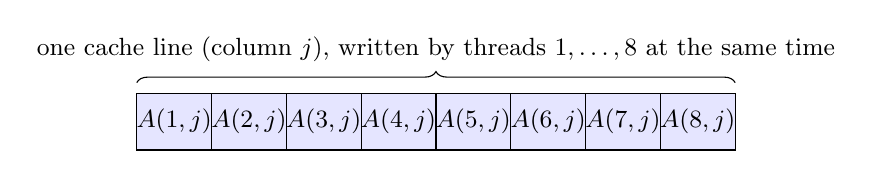
\begin{tikzpicture}[x=0.95cm,y=0.9cm]
  \foreach \i in {1,...,8} { \draw[fill=blue!10] (\i-1,0) rectangle (\i,0.8); \node at (\i-0.5,0.4) {\small $A(\i,j)$}; }
  \draw[decorate,decoration={brace,amplitude=4pt}] (0,0.95) -- (8,0.95) node[midway,above=4pt,font=\small]{one cache line (column $j$), written by threads $1,\dots,8$ at the same time};
\end{tikzpicture}
\end{center}

That is false sharing in its worst form.

\textbf{The slide's remedy.} Reorganise so that each thread works on a \emph{set of consecutive rows}. In a column, a block of consecutive rows
is contiguous in memory, so a thread's data forms long contiguous runs and different threads' runs only meet at the block boundaries.
A boundary can still fall inside a line (``overlapping of cache lines if matrix size not divisible by processors''). \emph{Padding} fixes this: add
dummy elements so the block size is a multiple of the line size.

\begin{workedex}{padding the number of rows}
A matrix has $n=100$ rows of doubles ($8$ bytes), $p=4$ threads, $64$-byte lines (8 doubles per line), and the array starts on a line boundary.
\begin{itemize}
  \item Without padding: each thread gets $25$ rows, which is $200$ bytes $=3.125$ lines. The block boundaries fall inside lines, so
        neighbouring threads share lines. (Moreover a column is $800$~bytes $=12.5$ lines, so columns are not line-aligned either.)
  \item With padding: round the per-thread block up to a multiple of $8$ rows, $25\to 32$, and allocate $4\times 32 = 128$ rows
        (the last $28$ rows are dummy). Each thread's block is $256$ bytes $=4$ whole lines and a column is $1024$~bytes
        $=16$ lines, so each column starts on a line boundary and no line is shared between threads.
\end{itemize}
The price is $28\%$ extra memory; padding trades memory for speed. The same idea applies to C, with the roles of rows and columns swapped.
\end{workedex}

\begin{keyidea}
Coherence works on \emph{lines}. To avoid false sharing, give each thread data that is contiguous and (if possible) aligned to line boundaries,
and keep frequently written per-thread data in private variables instead of neighbouring slots of a shared array. Tools such as Linux
\cl{perf c2c} can detect it.
\end{keyidea}

\section*{Exercises}
\addcontentsline{toc}{section}{Exercises}
\begin{enumerate}[label=\textbf{\thechapter.\arabic*},leftmargin=*]
  \item Three processors $P_1,P_2,P_3$ all start with a line in state I. Using the three-state protocol, give the state of the line in each
        cache after each step: (a) $P_1$ writes; (b) $P_2$ reads; (c) $P_2$ writes; (d) $P_3$ reads; (e) $P_1$ reads.
  \item $P_1$ writes a variable $50$ times in a row, then $P_2$ reads it once. Count the bus transactions under write-update
        and under write-invalidate (count each broadcast, invalidation and read miss as one).
  \item A system has $256$ processors and $128$-byte cache lines. What is the percentage overhead of a full bit-vector directory?
  \item Four threads each increment their own \cl{int} counter, stored in \cl{int c[4]}. How many cache lines hold the array
        (assume it is $64$-byte aligned)? How much would you pad each counter, and how much memory would the padded array use?
  \item Explain why read-only shared data causes no coherence traffic after the first misses.
  \item A column-major matrix has $n=100$ rows, $p=8$ threads and $64$-byte lines. Following the slide's approach,
        choose the padded number of rows.
\end{enumerate}